% python classes slides - classes_introduction
% (c) 2012 Kostiantyn Danylov aka koder 
% koder.mail@gmail.com
% distributed under CC-BY licence
% http://creativecommons.org/licenses/by/3.0/deed.en

\documentclass{article}
% XeLaTeX
\usepackage{xltxtra}
\usepackage{xunicode}
\usepackage{listings}
\usepackage[landscape]{geometry}

% Fonts
\setmainfont{DejaVu Sans} %{Arial}
\newfontfamily\cyrillicfont{Nimbus Roman No9 L} %{Arial}
\setmonofont{Courier New}
%\setmonofont{Ubuntu Mono}

%\setmonofont{DejaVu Sans Mono}

% Lang
\usepackage{polyglossia}
\setmainlanguage{russian}
\setotherlanguage{english}
\usepackage[dvipsnames,table]{xcolor}


\ifx\pdfoutput\undefined
\usepackage{graphicx}
\else
\usepackage[pdftex]{graphicx}
\fi

\lstset{
	language=python,
	keywordstyle=\color{Emerald},%\texttt, 
	commentstyle=\color{OliveGreen},%\texttt,
	stringstyle=\color{Bittersweet},%\texttt,
	tabsize=4,
	numbers=left,
	xleftmargin=10pt,
	morekeywords={with,as},	
	numberstyle=\large,
	%identifierstyle=\texttt,
	%basicstyle=\texttt,
}

\usepackage{hyperref}

\hypersetup{
	colorlinks=true,
	urlcolor=blue
}

\usepackage{float}
%\floatstyle{boxed} 
%\restylefloat{figure}
\usepackage[normalem]{ulem}

\input{files/python_cmds}

\begin{document}
\LARGE
%-------------------------------------------------------------------------------
\begin{center} Пример №1 \end{center}
    Написать функцию для вычисления среднего от массива чисел
\newpage

%-------------------------------------------------------------------------------
\begin{center} Среднее. Вариант №1 \end{center}
\begin{lstlisting}
    def mean(numbers):
        res = 0
        for num in numbers:
            res += num
        return nun / len(numbers)
\end{lstlisting}
\newpage

%-------------------------------------------------------------------------------
\begin{center} Нужно добавить поддержку рациональных чисел \end{center}
Рациональное число - пара (числитель, знаменатель). Будем передавать
рациональные числа в виде кортежа.

$$
\frac{a}{b} + \frac{c}{d} = \frac{ad + bc}{bd}\,\,;
\quad
\frac{a}{b} / c = \frac{a}{cd}
$$
\newpage

%-------------------------------------------------------------------------------
\begin{center} Среднее. Вариант №2 \end{center}
\begin{lstlisting}
    def mean(numbers):
        res = (0, 1)

        for num in numbers:
            if isinstance(num, int):
                num = (num, 1)

            res = (res[0] * num[1] + res[1] * num[0], 
                   num[1] * res[1])

        return (res[0], res[1] * len(numbers))
\end{lstlisting}
\newpage

%-------------------------------------------------------------------------------
\begin{center} Процедурный стиль - анализ \end{center}
\begin{itemize}
    \item \lstinline!if isinstance(num, int):! - ужасно и вызывает массу проблем
    \item Добавление новых типов требует изменения функции mean
    \item Перегрузка функций решает небольшую часть проблем
    \item Если mean в сторонней библиотеке - ничего не выйдет
    \item Дописать еще одну функцию и использовать ее - не выход
\end{itemize}
\begin{center} \includegraphics[scale=0.6]{images/code_structure.jpg} \end{center} 
\newpage

%-------------------------------------------------------------------------------
\begin{center} Процедурный стиль - причины неудачи \end{center}
\begin{itemize}
    \item На самом деле mean не нужно знать как устроенны данные внутри
    \item Ей нужно только знать как складывать и делить их
    \item Эта информация есть в той точке, где мы определяем новый тип
\end{itemize}
\newpage

%-------------------------------------------------------------------------------
\begin{center} Вариант №3 \end{center}
Передавать в mean вместе с данными функции для сложения и деления.
Хранить данные и функции будем в словаре.

\begin{lstlisting}
    def add_rational(x, y):
        return  (x['num'] * y['denom'] + \
                 x['denom'] * y['num'], 
                 x['denom'] * y['denom'])

    def div_rational(x, y):
        return (x['num'], x['denom'] * y)

    def mk_rational(num, denom):
        return {'num':num, 
                'denom':denom, 
                'add':add_rational, 
                'div':div_rational}

\end{lstlisting}
\newpage

%-------------------------------------------------------------------------------
\begin{center} Вариант №3 \end{center}
\begin{lstlisting}
    def mean(numbers):
        if isinstance(numbers[0], int):
            res = numbers[0]
            for num in numbers[1:]:
                res += num
            return res / len(numbers)
        else:
            res = numbers[0]
            for num in numbers[1:]:
                res = res['add'](res, num)
            return res['div'](res, len(numbers))

    res = mean([mk_rational(1, 3), 
                mk_rational(1, 2)])
\end{lstlisting}
\newpage

%-------------------------------------------------------------------------------
\begin{center} 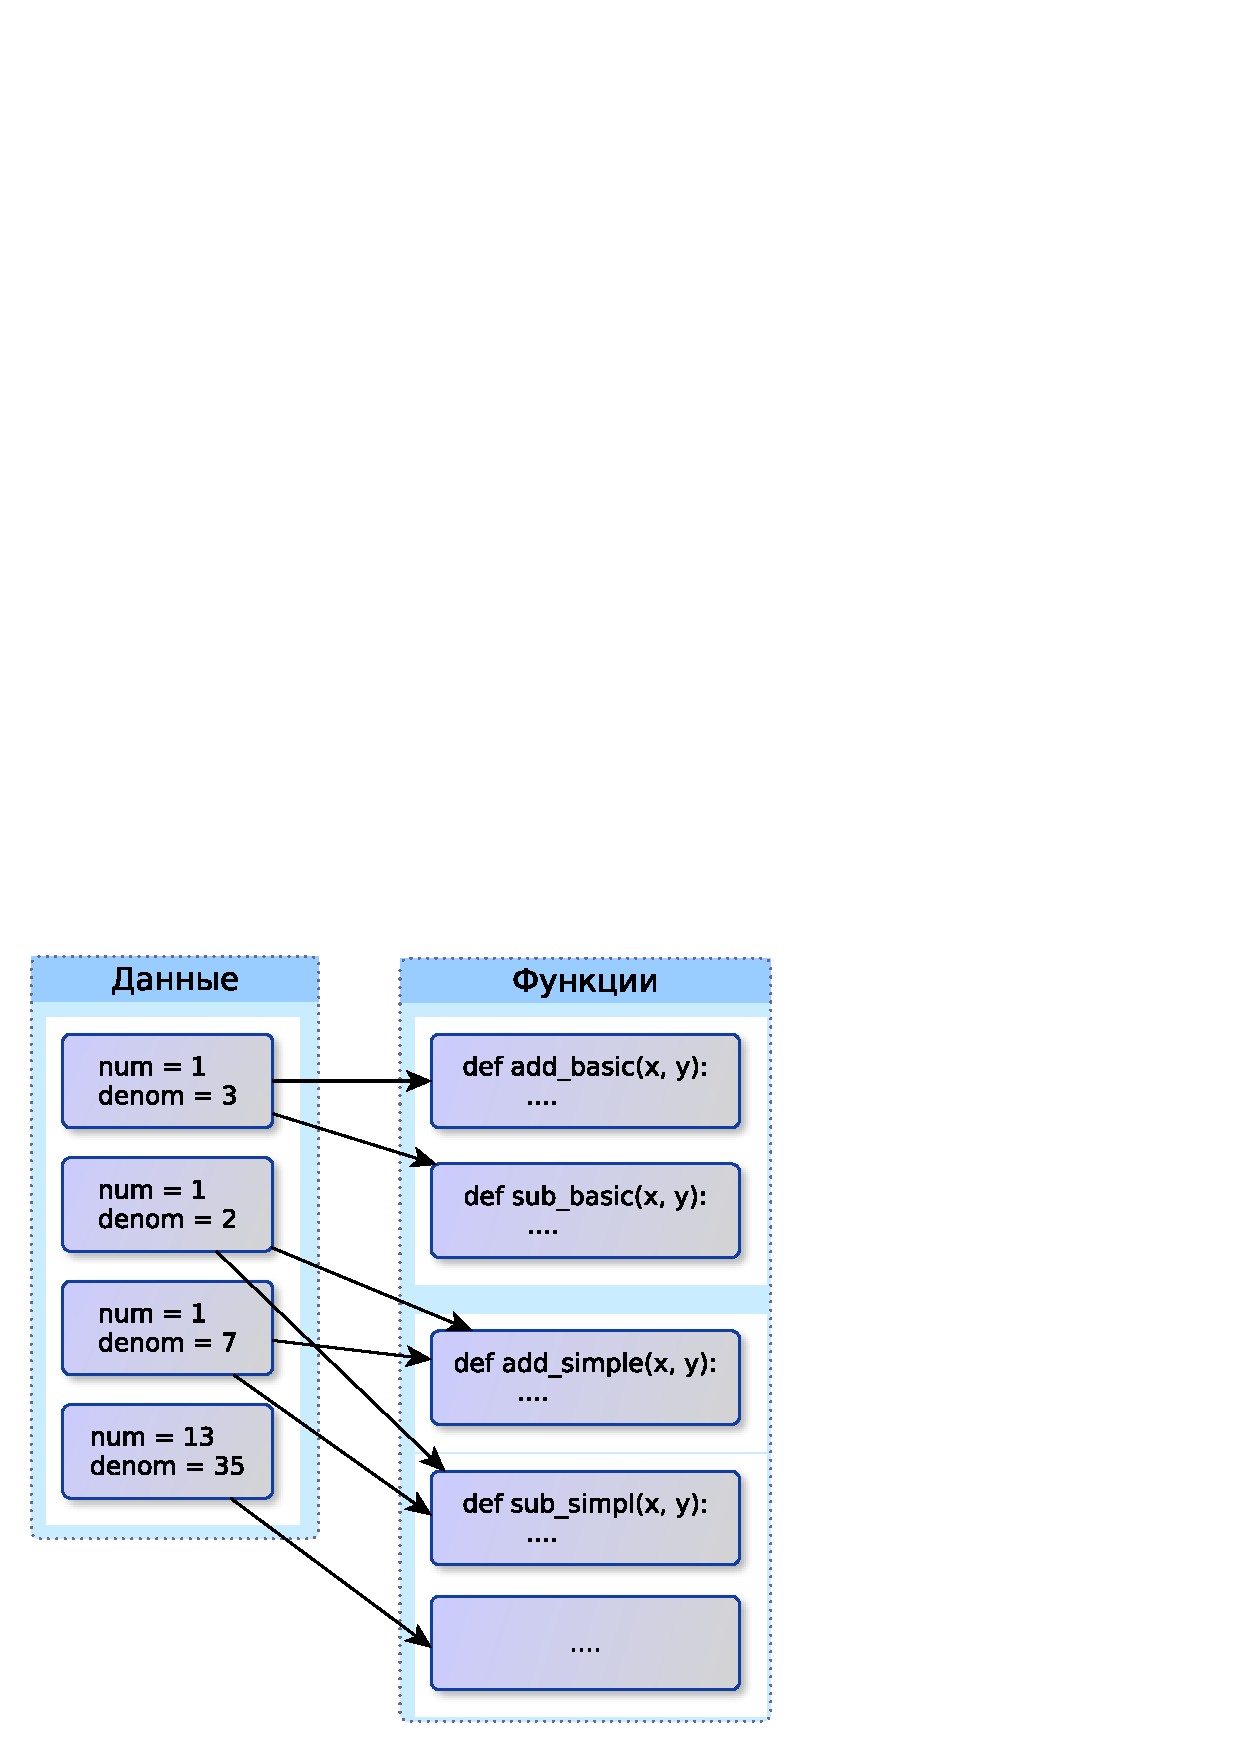
\includegraphics{images/semi_OOP_style.jpg} \end{center} 
\newpage

%-------------------------------------------------------------------------------
\begin{center} Нужно автоматически упрощать после операции 
    и добавить функцию для вычитания \end{center}
\begin{lstlisting}
    def mk_rational_auto_simpl(num, denom):
        return dict(num=num, 
                    denom=denom, 
                    add=add_rational_auto_simpl, 
                    div=div_rational_auto_simpl,
                    sub=sub_rational_auto_simpl)
\end{lstlisting}
\newpage

%-------------------------------------------------------------------------------
\begin{center} Немного измененный вариант \end{center}
\begin{lstlisting}
    def sub_rational_auto_simpl(x, y):
        nx = x['neg'](x)
        return x['add'](x, y)

    def mk_rational_auto_simpl(num, denom):
        res = mk_rational(num, denom)
        res['add'] = add_rational_auto_simpl
        res['div'] = div_rational_auto_simpl
        return res
\end{lstlisting}
\newpage

%-------------------------------------------------------------------------------
\begin{center} Не совсем процедурный стиль - анализ \end{center}
\begin{itemize}
    \item Кода стало больше
    \item Его расширение значительно упростилось - функции 
            могут обрабатывать данные, не зная их конкретного типа
    \item Тип - это операции, которые есть у него (duck tuping)
\end{itemize}
\newpage

%-------------------------------------------------------------------------------
\begin{center} Не совсем процедурный стиль - анализ \end{center}
\begin{itemize}
    \item Типовые теги иногда нужны.
    \item Каждый экземпляр содержит большое количество ссылок на одни и те же
          функции.
    \item Решение - вынесение всех методов в отдельный словарь, который все 
          переменные данного типа используют совместно. Одновременно этот
          словарь становится типовым тегом.
\end{itemize}
\newpage

%-------------------------------------------------------------------------------
\begin{center} Среднее. Вариант №4 \end{center}
\begin{lstlisting}
    RN = {'add': add_rational, 
          'sub': sub_rational,
          'div': div_rational,               
          'neg': neg_rational,               
          '__init__': mk_rational}

    ASRN = RN.copy()
    ASRN['add'] = add_rational_auto_simpl 
    ASRN['div'] = div_rational_auto_simpl 
    ASRN['__init__'] = add_rational_auto_simpl 

    x1 = BasicRN['__init__'](1, 2)
    x2 = ASRN['__init__'](1, 2)
\end{lstlisting}
\newpage

%-------------------------------------------------------------------------------
\begin{center}  Среднее. Вариант №4  \end{center}
\begin{lstlisting}
    def mean(numbers):
        if isinstance(numbers[0], int):
            ...
        else:
            res = numbers[0]
            for num in numbers[1:]:
                add_meth = res['__class__']['add']
                res = add_meth(res, num)

            div_meth = res['__class__']['div']
            return div_meth(res, len(numbers))
\end{lstlisting}
\newpage

%-------------------------------------------------------------------------------
\begin{center} Именно так и устроенно ООП \end{center}
\begin{itemize}
    \item Шаблон программирования, когда данные хранять ссылку на свой тип (класс)
    \item Тип хранит ссылки на реализации операций для себя
    \item А логика программы использует эти операции вместо прямой работы с данными
    \item Всё - объекты с интерфейсами (iter, число)
\end{itemize}
\newpage

%-------------------------------------------------------------------------------
\begin{center} Buzzwords \end{center}
\begin{itemize}
    \item Класс - тип данных, в котором есть методы
    \item Методами - функции в классе
    \item Экземпляры - объект конкретного класса
    \item Объект - экземплят какого либо класса*
    \item Атрибутами  - переменные внутри экземпляра
    \item Интерфейсом - набор методов и атрибутов
    \item Инкапсуляция - сокрытие внутренней структуры данных за методами
    \item Наследование - возможность использовать некоторый класс в качестве "базового"
    \item Полиморфизм - позможность изменить часть методов в базовом классе
    \item Перегрузка - изменение метода в дочернем классе
\end{itemize}
\newpage

%-------------------------------------------------------------------------------
\begin{center} 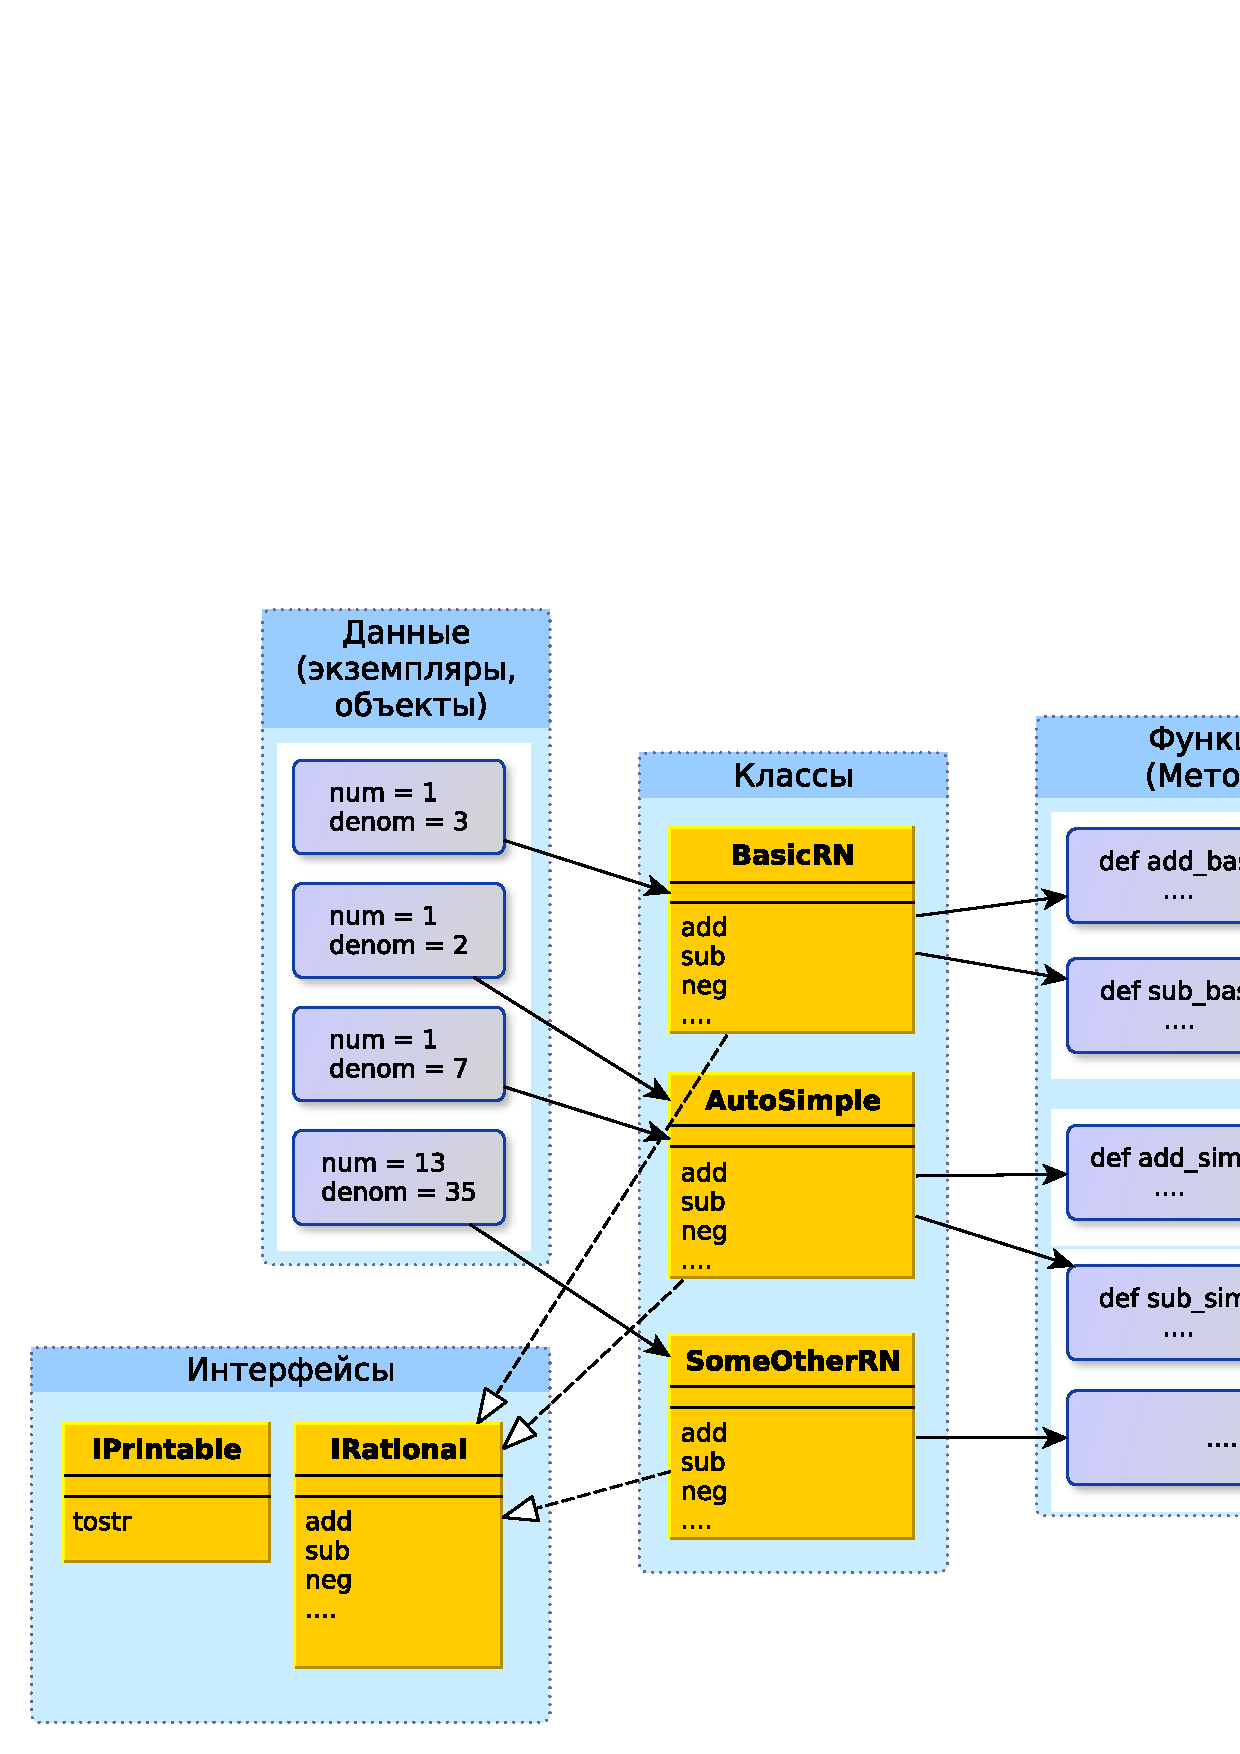
\includegraphics[scale=0.8]{images/oop_style.jpg} \end{center} 
\newpage

%-------------------------------------------------------------------------------
\begin{center} \includegraphics[scale=0.8]{images/interfaces.jpg} \end{center} 
\newpage

%-------------------------------------------------------------------------------
\begin{center} 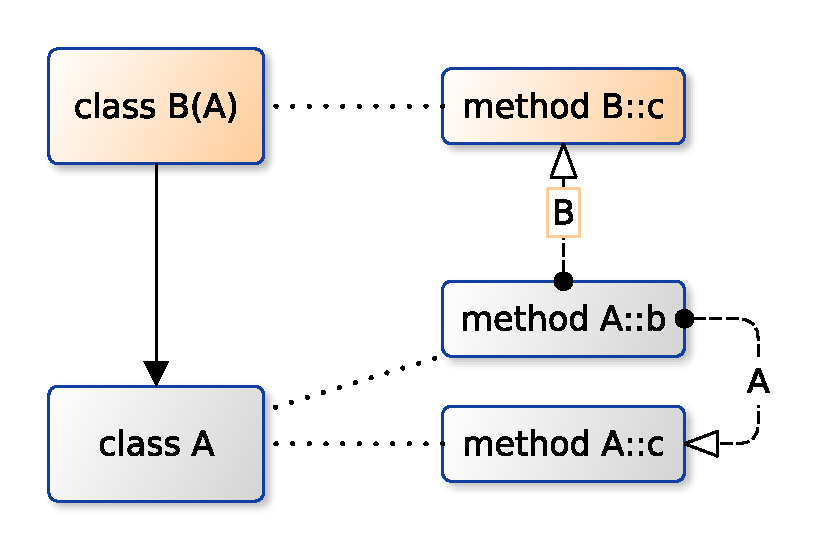
\includegraphics{images/virt_hierarchi.eps} \end{center} 
\newpage

%-------------------------------------------------------------------------------
\begin{center} Рациональные числа - классы \end{center}
\begin{lstlisting}
    class BasicRational(object):
        "basic rational number"
        def __init__(self, num, denom):
            self.num = num
            self.denom = denom

        def add(self, y):
            nd = self.denom * y.denom
            nn = self.num * y.denom + \
                 y.num * self.denom
            return BasicRational(nn, nd)

        def neg(self):
            return BasicRational(-self.num,
                                 self.denom)

        def sub(self, y):
            return self.add(y.neg())
\end{lstlisting}
\newpage

%-------------------------------------------------------------------------------
\begin{center} Объект в питоне \end{center} 
\begin{center} 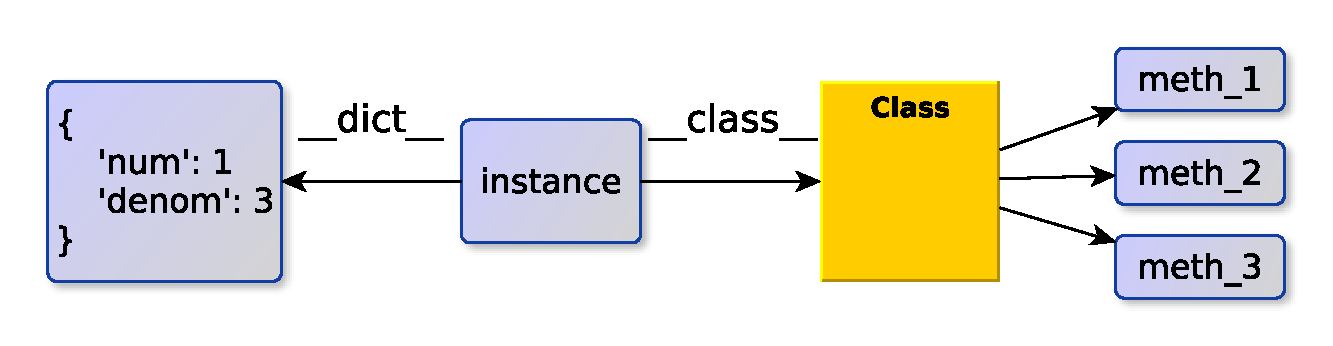
\includegraphics[scale=0.8]{images/python_instance.eps} \end{center} 
\lstinline!obj.__class__ == type(obj)! - класс объекта \\
\lstinline!obj.__dict__! - словарь, содержащий атрибуты объекта
\newpage

%-------------------------------------------------------------------------------
\begin{center} ООП без классов еще раз \end{center}
\begin{figure}[ht]
\begin{minipage}[b]{0.45\linewidth}
\large
\begin{lstlisting}
X = Y.copy()

def mk_X(val):
    res = mk_Y()
    res['val'] = val
    res['__class__'] = X
    return res

def tostr_X(x):
    return "X<val={}>".format(x['val'])

X = {'tostr' : tostr_X,
     '__init__': mk_X}

x = mk_X(1)

def print_list(lst):
    vals =  (obj['__class__']\
                    ['tostr'](obj)
                for obj in lst)
    return "[{}]".format(
            ", ".join(vals))
\end{lstlisting}
\end{minipage}
\hspace{2cm}
\begin{minipage}[b]{0.45\linewidth}
\large
\begin{lstlisting}
class X(Y):
 
    def __init__(self, val):
        Y.__init__(self)
        self.val = val



    def tostr(self):
        return "X<val={}>".format(self.val)




x = X(1)

def print_list(lst):
    vals =  (obj.tostr() 
                for obj in lst)
    
    return "[{}]".format(
        ", ".join(vals))
\end{lstlisting}
\end{minipage}
\end{figure}
\newpage

%-------------------------------------------------------------------------------
\begin{center} В BasicRational - ошибка \end{center}
\newpage

%-------------------------------------------------------------------------------
\begin{center} В BasicRational - ошибка \end{center}
\begin{lstlisting}
    def neg(self):
        return BasicRational(-self.num,
                             self.denom)


    def neg(self):
        return self.__class__(-self.num,
                               self.denom)
\end{lstlisting}
То же и в BasicRational.add
\newpage

%-------------------------------------------------------------------------------
\begin{center} Рациональные числа - классы \end{center}
\begin{lstlisting}
    x['__class__']['add'](x, y) == x.add(y) 
    # == BasicRational.add(x, y)
    x['num'] == x.num
    x['__class__']['add'](x, ...) == x.add
\end{lstlisting}
\newpage

%------------------------------------------------------------------------------
\begin{center} Среднее. Вариант №5 \end{center}
\begin{lstlisting}
    def mean(numbers):
        if isinstance(numbers[0], int):
            ...
        else:
            res = numbers[0]
            for num in numbers[1:]:
                res = res.add(num)

            return res.div(len(numbers))
\end{lstlisting}
\newpage

%------------------------------------------------------------------------------
\begin{center} Среднее. Вариант №6 \end{center}
Можно перегрузить операторы.
\begin{lstlisting}
    def mean(numbers):
        res = numbers[0]
        for num in numbers[1:]:
            res += num
        return res / len(numbers)
\end{lstlisting}
На самом деле эта функция работает для int, float, complex потому что
они тоже перегружают операторы типа object.
\newpage

%-------------------------------------------------------------------------------
\begin{center} ООП - в чем причина? \end{center}
\begin{itemize}
    \item Дополнительный уровень косвенности
    \item Написав add таким образом мы получили возможность 
            менять ее работу не трогая код
    \item Код, который создает новую дробь знает 
            подробности того, как с ней работать
    \item Код, который ее использует - не всегда
    \item Отделяя основной алгоритм функции от особенностей конкретных типов
          мы можем сделать ее гораздо более универсальной
\end{itemize}
\newpage

%-------------------------------------------------------------------------------
\begin{center} Пример №2 \end{center}
Необходимо сравненивать файлы одинаковой длинны посимвольно 
    и возвращать массив отличающихся позиций
\begin{lstlisting}
    def compare(fname1, fname2):
        res = []
        with open(fname1) as fd1:
            with open(fname2) as fd2:
                x1 = fd1.read(1)
                x2 = fd2.read(1)
                pos = 0
                while x1 != '':
                    if x1 != x2 :
                        res.append(pos)
                    x1 = fd1.read(1)
                    x2 = fd2.read(1)
                    pos += 1
        return res
\end{lstlisting}
\newpage

%-------------------------------------------------------------------------------
\begin{center} Пример №2 \end{center}
Необходимо сравненивать файлы посимвольно и возвращать массив отличающихся блоков
\begin{lstlisting}
    def compare_streams(iter1, iter2, cmp, on_diff):
        it = enumerate(izip(iter1, iter2))
        for pos, (ch1, ch2) in it:
            if cmp(x1, x2) != 0 :
                on_diff(pos)

    def compare_files(fname1, fname2):
        res = []
        with open(fname1) as fd1:
            with open(fname2) as fd2:
                compare_streams(fd1, fd2, cmp, res.append)
        return res
\end{lstlisting}
\newpage

%-------------------------------------------------------------------------------
\begin{center} Пример №2 \end{center}
\begin{itemize}
    \item Теперь compare\_streams может использоваться для сравнения любых последовательностей
    \item Как символьных, так и нет
    \item Можно сделать сравнение нечуствительным к регистру
    \item И для асинхронных потоков
    \item Все это очень полезно для создания повторно используемого кода
    \item Не всегда нужно передавать классы, часто достаточно функции. 
            В python точно. В C++ через шаблоны и std::function<>.
    \item Но только для повторно используемого - 
            \href{http://ru.wikipedia.org/wiki/%D0%9F%D1%80%D0%B8%D0%BD%D1%86%D0%B8%D0%BF_YAGNI}{YAGNI}
\end{itemize}
\newpage

%-------------------------------------------------------------------------------
\begin{center} Пример №3 \end{center}
    Написать обработчик выражения, состоящего из -, +, скобок и чисел.
    В первую очередь нас интересует вычислитель.
    (Пусть у нас уже есть синтаксический анализатор выражения - функция parse).
\begin{lstlisting}
    expression = "1 + 2 + ( 4 - 3 )"
    #pexpr = parse(expression)
    pexpr  = ('+', 
                 ('+', 1, 2), 
                 ('-', 3 , 4))
\end{lstlisting}
    \begin{center} 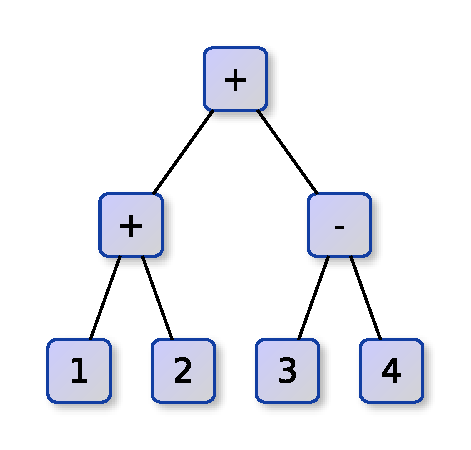
\includegraphics{images/parse_tree.eps} \end{center}     
\newpage

%-------------------------------------------------------------------------------
\begin{center} Решение №1 \end{center}
\begin{lstlisting}
    def evaluate(val):
        if isinstance(val, int):
            res = val
        else:
            operator, oper1, oper2 = val
            assert operator in "+-", \
                "Unknown operator " + operator

            v1 = evaluate(oper1)
            v2 = evaluate(oper2)

            if operator == '+':
                res = v1 + v2
            elif operator == '-':
                res = v1 - v2

        return res
\end{lstlisting}
\newpage

%-------------------------------------------------------------------------------
\begin{center} Добавить в выражение поддержку * и / \end{center}
\newpage

%-------------------------------------------------------------------------------
\begin{center} Добавить в выражение поддержку * и / \end{center}
\begin{lstlisting}
    class Operator(object):
        def evaluate(self, op1, op2):
            pass

    class Add(object):
        def evaluate(self, op1, op2):
            return op1 + op2

    class Mul(object):
        def evaluate(self, op1, op2):
            return op1 * op2

    expr = (Add(), (Add(), 1, 2), (Sub(), 3 , 4))
\end{lstlisting}
\newpage

%-------------------------------------------------------------------------------
\begin{center} Добавить в выражение поддержку * и / \end{center}
\begin{lstlisting}
    def evaluate_add(op1, op2):
        return op1 + op2

    def evaluate_mul(op1, op2):
        return op1 * op2

    expr = (evaluate_add,
                (evaluate_add, 1, 2), 
                (evaluate_mul, 3 , 4))
\end{lstlisting}
\newpage

%-------------------------------------------------------------------------------
\begin{center} Добавить в выражение поддержку * и / \end{center}
\begin{lstlisting}
    def evaluate(val):
        if isinstance(val, int):
            res = val
        else:
            operator, oper1, oper2 = val

            v1 = evaluate(oper1)
            v2 = evaluate(oper2)
            
            res = operator(v1, v2)
            #res = operator.evaluate(v1, v2)

        return res
\end{lstlisting}
\newpage

%-------------------------------------------------------------------------------
\begin{center} Добавить в выражение поддержку строк \end{center}
\newpage

%-------------------------------------------------------------------------------
\begin{center} Добавить в выражение поддержку строк \end{center}
\begin{lstlisting}
    class Value(object):
        def add(self, v2):
            pass

    class Int(Value):
        def __init__(self, val):
            self.val = val

        def add(self, v2):
            if isinstance(v2, int):
                return v2 + self.val
            else:
                return v2.add(self.val)

    def evaluate_add(op1, op2):
        return op1.add(op2)
\end{lstlisting}
\newpage

%-------------------------------------------------------------------------------
\begin{center} Проблемы? \end{center}
\newpage

%-------------------------------------------------------------------------------
\begin{center} Проблемы? \end{center}
Фукция parse. Почему?
\newpage

%-------------------------------------------------------------------------------
\begin{center} parse \end{center}
\begin{itemize}
    \item С одной стороны она должны явно знать какие типы создавать
    \item С другой стороны она не может этого знать
    \item Нужно передавать parse снаружи.
\end{itemize}
\newpage

%-------------------------------------------------------------------------------
\begin{center} Когда ООП \end{center}
\begin{itemize}
    \item Если есть участок кода, требующий определенного ограниченного 
          набора операций над входными данными
    \item Одновременно в программе могут быть несколько видов подходящих данных, 
          с различной функциональностью для реализации этого интерфейса
    \item Причем участок кода в свою очередь может быть одним из методов класса.
    \item Или группировки функций с общим глобальным состоянием
\end{itemize}
\newpage

%-------------------------------------------------------------------------------
\begin{center} Классы не предназначен для \end{center}
\begin{itemize}
    \item Группировки функций
    \item Группировки одной функции
    \item Если вы, ессно, используете нормальный ЯП
\end{itemize}
\newpage

%-------------------------------------------------------------------------------
\begin{center} ООП vs Процедурный стиль \end{center}
\begin{itemize}
    \item (-) Часто больше кода
    \item (-) Добавление нового метода требует нелокальных изменений
    \item (-) Замедляет работу
    \item (-) Усложняет язык
    \item (-) Логика размазывается
    \item (-) Разработка ООП дизайна требует больших навыков и времени, чем процедурного
    \item (-) Работает только если функция выбирается по типу одного параметра
\end{itemize}
\newpage

%-------------------------------------------------------------------------------
\begin{center} ООП vs Процедурный стиль \end{center}
\begin{itemize}
    \item (+) Уменьшает пересечение имен
    \item (+) Код лучше структурирован
    \item (+) Избавляет от ручной проверки типов
    \item (+) Избавляет от знания конкретного типа данных
    \item (+) Во многих случаях значительно упрощает расширение
              Позволяя корректно написанному коду работать с новыми типами данных
    \item (+) Более высокий уровень абстракции упрощает построение программы
              путем выделения стандартных шаблонов проектирования
    \item (+) Многие из идей ООП имеют прямую поддержку в языке
\end{itemize}
\newpage

%-------------------------------------------------------------------------------
\begin{center} Добавление нового метода требует нелокальных изменений : решение \end{center}
\begin{lstlisting}
    def to_xml(obj):
        if isinstance(obj, int):
            ...
        elif isinstance(obj, str):
            ...
        else:
            res = obj.to_xml()
        return res
\end{lstlisting}
\newpage

%-------------------------------------------------------------------------------
\begin{center} Проблема \end{center}
    \lstinline|x.add(y) != y.add(x)|. При других типах может быть совсем не верно. \\
    В чем проблема? Как решать?
\newpage

%-------------------------------------------------------------------------------
\begin{center} Проблема \end{center}
    \lstinline|x.add(y) != y.add(x)|. При других типах может быть совсем не верно. \\
    В чем проблема? Как решать? \\
    Нужна перегрузка add по обеим параметрам, что-то типа
    \lstinline!(x,y).add(x,y)!.  Классическое ООП не предлагает решения.
\newpage

%-------------------------------------------------------------------------------
\begin{center} Почти решение \end{center}
\begin{lstlisting}
    class X(Y):
        def add(self, y, final=False):
            if isinstance(y, Y):
                self.do_add_Y(y)
            elif isinstance(y, X):
                self.do_add_X(y)
            else:
                return y.add(self, True)
\end{lstlisting}
Более-менее работает для линейных иерархий.
\newpage

%-------------------------------------------------------------------------------
\begin{center} Но для не линейных... \end{center}
    \begin{center} \includegraphics[scale=0.9]{images/virtual_problem.jpg} \end{center}
\newpage

%-------------------------------------------------------------------------------
\begin{center} Альтернативы \end{center}
\begin{itemize}
    \item CLOS - возможность расширять работу функции после ее создания,
          динамически подключая новые реализации
    \item Функция превращается в объект-хранилище шаблонов со ссылками на реализации
    \item Позволяет перегружать поведение не только по одному параметру
    \item Замедляет работу
\end{itemize}
\begin{center} 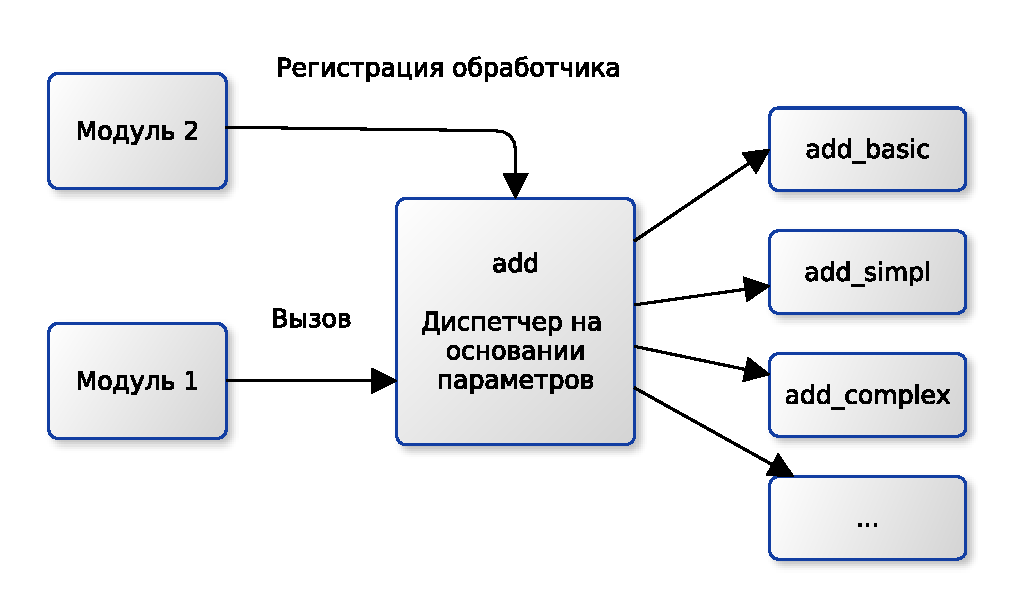
\includegraphics[scale=0.8]{images/CLOS.eps} \end{center} 
\newpage

%-------------------------------------------------------------------------------
\begin{center} Альтернативы \end{center}
\begin{itemize}
    \item Аспектное программирование
    \item \href{PEAK-Rules}{http://pypi.python.org/pypi/PEAK-Rules}
\end{itemize}
\newpage

%-------------------------------------------------------------------------------
\end{document}
